\documentclass[11pt]{article}

%%TO EDIT
\newcommand{\dueclassnumber}{3}
\newcommand{\assignmentnum}{1}

% CHANGE issolution{0} to issolution{1} for homework submission.
% WRITE solutions inside the \solution{} commands.
% or, you can use \if\issolution1 … \fi

\def\issolution{1}
\def\myname{Allen Liu} % My name goes here
\def\mysec{01} % Section number goes here
\def\myCM{374} % Campus Mailbox goes here

\input{../common/flags}

% Leave the next line alone. This is for my answer keys.
%\def\isanswerkey{1}

\usepackage{bbm,fancyhdr,ifthen,setspace,hyperref,url}
\usepackage{amssymb,amsmath,enumitem,amsthm,mathrsfs}
\usepackage{graphicx,xspace,color}
\usepackage{hhline}
\usepackage{tikz}
\usetikzlibrary{automata, positioning, arrows,chains,scopes,fit}
\tikzset{
->, % makes the edges directed
>=stealth', % makes the arrow heads bold
node distance=2.4cm, % specifies the minimum distance between two nodes. Change if necessary.
every state/.style={thick, fill=gray!10}, % sets the properties for each ’state’ node
initial text=$ $, % sets the text that appears on the start arrow
}

\topmargin=-.5in
\headsep=0.0in
\oddsidemargin=-.35in
\evensidemargin=-.65in
\textwidth=7.25in
\textheight=9.75in
\footskip=0in
\usepackage{titlesec}
\titlespacing*{\paragraph}{0pt}{2ex plus 1ex minus .2ex}{1ex}
\fancyhf{} % clear all header and footers
\renewcommand{\headrulewidth}{0pt} % remove the header rule
%\rfoot{\thepage}
\pagestyle{fancy}

\ifx\myname\undefined
\def\myname{}
\fi

\ifx\isanswerkey\undefined
\def\isanswerkey{0}
\fi

\if\isanswerkey1
\def\issolution{1}
\fi


\newcommand{\getcourseyear}[1]{2022}
\newcommand{\getcourseterm}{Spring \getcourseyear{1}}

\newcommand{\getclassmonthnum}[1]{\ifthenelse{#1<16}{3}{\ifthenelse{#1<29}{4}{5}}}
\newcommand{\getclassmonthshort}[1]{\ifthenelse{#1<16}{Mar}{\ifthenelse{#1<29}{Apr}{May}}}
\newcommand{\getclassmonth}[1]{\ifthenelse{#1<16}{March}{\ifthenelse{#1<29}{April}{May}}}
\newcommand{\getclassdayofmonth}[1]{\ifthenelse{
#1=1}{7}{\ifthenelse{
#1=2}{8}{\ifthenelse{
#1=3}{10}{\ifthenelse{
#1=4}{11}{\ifthenelse{
#1=5}{14}{\ifthenelse{
#1=6}{15}{\ifthenelse{
#1=7}{17}{\ifthenelse{
#1=8}{18}{\ifthenelse{
#1=9}{21}{\ifthenelse{
#1=10}{22}{\ifthenelse{
#1=11}{24}{\ifthenelse{
#1=12}{25}{\ifthenelse{
#1=13}{28}{\ifthenelse{
#1=14}{29}{\ifthenelse{
#1=15}{31}{\ifthenelse{
#1=16}{1}{\ifthenelse{
#1=17}{4}{\ifthenelse{
#1=18}{5}{\ifthenelse{
#1=19}{7}{\ifthenelse{
#1=20}{8}{\ifthenelse{
#1=21}{18}{\ifthenelse{
#1=22}{19}{\ifthenelse{
#1=23}{21}{\ifthenelse{
#1=24}{22}{\ifthenelse{
#1=25}{25}{\ifthenelse{
#1=26}{26}{\ifthenelse{
#1=27}{28}{\ifthenelse{
#1=28}{29}{\ifthenelse{
#1=29}{2}{\ifthenelse{
#1=30}{3}{\ifthenelse{
#1=31}{5}{\ifthenelse{
#1=32}{6}{\ifthenelse{
#1=33}{9}{\ifthenelse{
#1=34}{10}{\ifthenelse{
#1=35}{12}{\ifthenelse{
#1=36}{13}{\ifthenelse{
#1=37}{16}{\ifthenelse{
#1=38}{17}{\ifthenelse{
#1=39}{19}{\ifthenelse{
#1=40}{20}{}}}}}}}}}}}}}}}}}}}}}}}}}}}}}}}}}}}}}}}}}

\newcommand{\getclassdate}[1]{\getclassmonth{#1}\xspace\getclassdayofmonth{#1}}
\newcommand{\getclassdateshort}[1]{\getclassmonthshort{#1}\xspace\getclassdayofmonth{#1}}
\newcommand{\getclassdatenum}[1]{\getclassmonthnum{#1}/\getclassdayofmonth{#1}}
\newcommand{\getMday}{Mon}
\newcommand{\getTday}{Tue}
\newcommand{\getWday}{Wed}
\newcommand{\getRday}{Thu}
\newcommand{\getFday}{Fri}
\newcommand{\getclassdayofweek}[1]{\ifthenelse{
#1=1}{\getMday}{\ifthenelse{#1=2}{\getTday}{\ifthenelse{#1=3}{\getRday}{\ifthenelse{#1=4}{\getFday}{\ifthenelse{
#1=5}{\getMday}{\ifthenelse{#1=6}{\getTday}{\ifthenelse{#1=7}{\getRday}{\ifthenelse{#1=8}{\getFday}{\ifthenelse{
#1=9}{\getMday}{\ifthenelse{#1=10}{\getTday}{\ifthenelse{#1=11}{\getRday}{\ifthenelse{#1=12}{\getFday}{\ifthenelse{
#1=13}{\getMday}{\ifthenelse{#1=14}{\getTday}{\ifthenelse{#1=15}{\getRday}{\ifthenelse{#1=16}{\getFday}{\ifthenelse{
#1=17}{\getMday}{\ifthenelse{#1=18}{\getTday}{\ifthenelse{#1=19}{\getRday}{\ifthenelse{#1=20}{\getFday}{\ifthenelse{
#1=21}{\getMday}{\ifthenelse{#1=22}{\getTday}{\ifthenelse{#1=23}{\getRday}{\ifthenelse{#1=24}{\getFday}{\ifthenelse{
#1=25}{\getMday}{\ifthenelse{#1=26}{\getTday}{\ifthenelse{#1=27}{\getRday}{\ifthenelse{#1=28}{\getFday}{\ifthenelse{
#1=29}{\getMday}{\ifthenelse{#1=30}{\getTday}{\ifthenelse{#1=31}{\getRday}{\ifthenelse{#1=32}{\getFday}{\ifthenelse{
#1=33}{\getMday}{\ifthenelse{#1=34}{\getTday}{\ifthenelse{#1=35}{\getRday}{\ifthenelse{#1=36}{\getFday}{\ifthenelse{
#1=37}{\getMday}{\ifthenelse{#1=38}{\getTday}{\ifthenelse{#1=39}{\getRday}{\ifthenelse{#1=40}{\getFday}\xspace
}}}}}}}}}}}}}}}}}}}}}}}}}}}}}}}}}}}}}}}}
\newcommand{\examdate}[1]{\ifthenelse{#1=1}{March 23, \getcourseyear{11}}{\ifthenelse{#1=2}{April 7, \getcourseyear{11}}{\ifthenelse{#1=3}{May 4, \getcourseyear{11}}{\ifthenelse{#1=4}{ } {}}}}}




\newcommand{\classdate}[1]{\getclassdate{#1}, \getcourseyear{#1}}
\newcommand{\dueclassdate}{\getclassdayofweek{\dueclassnumber} \getclassdateshort{\dueclassnumber}}


\newcommand\largeemptyspace{\vphantom{\textnormal{$\ds\int$}}}
\newcommand\nameblank{\if\issolution0\underline{\hskip11.25cm {\largeemptyspace}}
  \else\underline{\hskip.2cm{\LARGE\myname}\hskip6cm}\fi}
\newcommand\nameblankshort{\if\issolution0\underline{\hskip9.5cm {\largeemptyspace}}
  \else\underline{\hskip.2cm{\LARGE\myname {\largeemptyspace}}\hskip.2cm}\fi}
\newcommand\secblank{\if\issolution0\underline{\hskip1.5cm{\largeemptyspace}}
  \else\underline{\hskip.2cm{\LARGE\mysec {\largeemptyspace}}\hskip.2cm} \hskip.8cm \fi}
\newcommand\CMblank{\if\issolution0\underline{\hskip2.25cm{\largeemptyspace}}
  \else\underline{\hskip.2cm{\LARGE\myCM {\largeemptyspace}}\hskip.2cm}\fi}

\newcommand{\namegroupline}{Name: \nameblank Group \#: \underline{\hskip1.5cm{\largeemptyspace}}}
\newcommand{\nameline}{\begin{minipage}{0.6\linewidth} Name: \nameblank \end{minipage}}
\newcommand{\namelineshort}{Name: \nameblankshort}
\newcommand{\namesecline}{\begin{minipage}{0.7\linewidth} Name: \nameblank \end{minipage} \hfill \begin{minipage}{0.29\linewidth}Section \#: \secblank\end{minipage}}
\newcommand{\namesecCMline}{\begin{minipage}{0.6\linewidth}Name: \nameblankshort \end{minipage} \hfill \begin{minipage}{0.4\linewidth} Section \# \secblank CM\# \CMblank \end{minipage}}
\newcommand{\keyline}{{\color{red} SOLUTION KEY}}
%\newcommand{\nameline}{Name: \rule{11.5cm}{0.01cm} \hfill Section: \rule{1.5cm}{0.01cm}}
%\newcommand{\keyline}{Name: \rule{4cm}{0.01cm} SOLUTION KEY \rule{4cm}{0.01cm} \hfill Section: \rule{1.5cm}{0.01cm}}
%\newcommand{\groupline}{Group members present: \rule{8.5cm}{0.01cm} \hfill Group \#: \rule{1.5cm}{0.01cm}}
\newcommand{\course}{CSSE/MA 474\xspace}
\newcommand{\coursewithname}{CSSE/MA 474. Theory of Computation\xspace}


\newcommand{\wtitlestuff}{
\if\isanswerkey0
  \nameline
  \else
  \keyline
\fi
\begin{center}
\large \course Worksheet for Class \#\classnumber\\
\small \classdate{\classnumber}
\normalsize
\end{center}}

\newcommand{\lectitlestuff}{
\begin{center}
\Large \course Lecture \#\classnumber\\
\vskip 3pt \small Nate Chenette \\ \classdate{\classnumber}
\normalsize
\end{center}}

\newcommand{\othertitlestuff}{
\begin{center}
\Large \othertitle\\
\small \coursewithname\\
Class \#\classnumber, \classdate{\classnumber}\\
\normalsize
\end{center}}

\newcommand{\othertitlestuffnodate}{
\begin{center}
\Large \othertitle\\
\small \coursewithname\\
\normalsize
\end{center}}

\newcommand{\othernametitlestuff}{
\nameline\\
\othertitlestuff
}

\newcommand{\assignmenttitlestuff}{
\begin{center}
\Large \course Assignment \assignmentnum\\
\small Due date: \dueclassdate
\normalsize
\end{center}}

\newcommand{\assignmentnametitlestuff}{
\if\isanswerkey0
  \namesecCMline
  \else
  \keyline
\fi
\assignmenttitlestuff
}

\newcommand{\quiznametitlestuff}{
\if\isanswerkey0
  \namesecCMline
  \else
  \keyline
\fi
\begin{center}
\Large \course Quiz \quiznum\\
\small \classdate{\classnumber}
\normalsize
\end{center}}


\setlength{\parindent}{0in}
\setlength{\fboxsep}{.1in}

\renewcommand{\emptyset}{\varnothing}
\newcommand{\tvs}{\textvisiblespace}
\newcommand{\brk}{\vskip.2cm \hrule \vskip.2cm}
\newcommand{\ds}{\displaystyle}
\newcommand{\abs}[1]{\left\lvert {#1}\right\rvert}
\newcommand{\Lsym}{\text{L}}
\newcommand{\Rsym}{\text{R}}
\newcommand{\qacc}{q_{\textnormal{accept}}}
\newcommand{\qrej}{q_{\textnormal{reject}}}
\newcommand{\tmRej}{$\to$ \textbf{\textit{reject}}}
\newcommand{\tmAcc}{$\to$ \textbf{\textit{accept}}}
\def\lep{\le_\textnormal{P}}
\def\lem{\le_\textnormal{m}}
\def\ATM{A_\textnormal{TM}}
\newcommand{\vv}[2]{\begin{bmatrix} {#1} \cr {#2} \end{bmatrix}}
\newcommand{\vvt}[2]{\begin{bmatrix} {\tt #1} \cr {\tt #2} \end{bmatrix}}
\def\hs{\quad \texttt\#\quad }
\def\multiset#1#2{\ensuremath{\left(\kern-.3em\left(\genfrac{}{}{0pt}{}{#1}{#2}\right)\kern-.3em\right)}}
\def\time{\textsf{TIME}}
\def\ntime{\textsf{NTIME}}
\def\P{\textsf{P}}
\def\NP{\textsf{NP}}
   
%logic
\newcommand{\se}{\big|}
\newcommand{\lra}{\leftrightarrow}
\newcommand{\Lra}{\Leftrightarrow}
\newcommand{\we}{\wedge}
\def\thf{%
   \leavevmode
   \lower0.2ex\hbox{$\cdot$}%
   \kern-0.0em\raise0.7ex\hbox{$\cdot$}%
   \kern-0.0em\lower0.2ex\hbox{$\cdot$}%
   \thinspace}

%Number Systems
\newcommand{\bbZ}{\mathbb{Z}}
\newcommand{\bfZ}{\mathbf{Z}}
\newcommand{\bfZp}{\mathbf{Z}^+}
\newcommand{\bbN}{\mathbb{N}}
\newcommand{\bfN}{\mathbf{N}}
\newcommand{\bbQ}{\mathbb{Q}}
\newcommand{\bfQ}{\mathbf{Q}}
\newcommand{\bbR}{\mathbb{R}}
\newcommand{\bfR}{\mathbf{R}}
\newcommand{\bbC}{\mathbb{C}}
\newcommand{\bfC}{\mathbf{C}}

%sets
\newcommand{\U}{\mathscr{U}}
\newcommand{\ol}[1]{\overline{#1}}
\newcommand{\ssq}{\subseteq}
\newcommand{\sst}{\subset}
\def\ps{\mathcal{P}}
\def\sd{\,\triangle\,}
\def\sdonly{\triangle}
\def\es{\emptyset}

%cards
\def\hst{\heartsuit}
\def\cst{\clubsuit}
\def\sst{\spadesuit}
\def\dst{\diamondsuit}


\newcommand{\lcm}{{\rm lcm}}


\newcommand{\imgdir}{../images/}


\newcommand{\makeexamcover}{
\ifdefined\finalexam
\ \vskip2cm
\begin{center}
\huge \course Final Exam \\
\Large \finalexamdate \vskip1cm
\end{center}
\normalsize \instructions \vskip1cm
\begin{spacing}{1.5}
\begin{center}
\scorechart
\end{center}
\end{spacing}
\else \ifdefined\examnum
\ \vskip2cm
\begin{center}
\huge \course Exam \examnum \\
\Large \examdate{\examnum} \vskip1cm
\end{center}
\normalsize \instructions \vskip1cm
\begin{spacing}{1.5}
\begin{center}
\scorechart
\end{center}
\end{spacing}
\fi
\fi
}




\fancypagestyle{examcover}{% 
\fancyhf{}
\renewcommand{\footrulewidth}{0pt}
\lhead{\if\isanswerkey1{\keyline}\else{\nameline}\fi}
%\lhead{\if\isanswerkey1{\keyline}\else{\namesecline}\fi}
}



\fancypagestyle{exameverypage}{% 
\fancyhf{}
\renewcommand{\footrulewidth}{0pt}
\rhead{\if\isanswerkey1{\keyline}\else{}\fi}
\fancyfoot[R]{\thepage}
%\lhead{\if\isanswerkey1{\keyline}\else{\namesecline}\fi}
}

\newcommand{\definition}[1]{{\sc Definition}.~~{#1}\vskip.2cm}

\usepackage[framemethod=default]{mdframed}
\global\mdfdefinestyle{red1}{linecolor=red, linewidth=1pt, leftmargin=1cm, rightmargin=1cm}
\global\mdfdefinestyle{black1}{linecolor=black, linewidth=1pt,} %leftmargin=.1cm, rightmargin=.1cm}

\newcommand{\solution}[2][]{\if\issolution0 #1 \else \begin{mdframed}[style=black1] #2 \end{mdframed} \fi}

\newcommand{\cmblanka}[1]{\if\issolution0 	\underline{\hskip1cm{\largeemptyspace}}
\else 						  		\underline{\hskip.35cm {#1}\hskip.35cm{\largeemptyspace}}\fi}
\newcommand{\sblanka}[1]{\if\issolution0 		\underline{\hskip1.5cm{\largeemptyspace}}
\else 						  		\underline{\hskip.25cm {#1}\hskip.25cm{\largeemptyspace}}\fi}
\newcommand{\mblanka}[1]{\if\issolution0 	\underline{\hskip3cm{\largeemptyspace}}
\else 						  		\underline{\hskip.5cm {#1}\hskip.5cm{\largeemptyspace}}\fi}
\newcommand{\lblanka}[1]{\if\issolution0 		\underline{\hskip4.5cm{\largeemptyspace}}
\else 						  		\underline{\hskip.75cm {#1}\hskip.75cm{\largeemptyspace}}\fi}
\newcommand{\Lblanka}[1]{\if\issolution0		\underline{\hskip6cm{\largeemptyspace}}
\else 								\underline{\hskip1cm {#1}\hskip1cm{\largeemptyspace}}\fi}
\newcommand{\LLblanka}[1]{\if\issolution0	\underline{\hskip7.5cm{\largeemptyspace}}
\else 								\underline{\hskip1.25cm {#1}\hskip1.25cm{\largeemptyspace}}\fi}
\newcommand{\LLLblanka}[1]{\if\issolution0 	\underline{\hskip9cm{\largeemptyspace}}
\else 								\underline{\hskip1.5cm {#1}\hskip1.5cm{\largeemptyspace}}\fi}
\newcommand{\tinyspacea}[1]{\if\issolution0 	\hskip.2cm{\largeemptyspace}
\else 						  		{#1}{\largeemptyspace}\fi}
\newcommand{\cmspacea}[1]{\if\issolution0 	\hskip1cm{\largeemptyspace}
\else 						  		\hskip.15cm {#1}\hskip.15cm{\largeemptyspace}\fi}
\newcommand{\sspacea}[1]{\if\issolution0 		\hskip1.5cm{\largeemptyspace}
\else 						  		\hskip.25cm {#1}\hskip.25cm{\largeemptyspace}\fi}
\newcommand{\mspacea}[1]{\if\issolution0 	\hskip3cm{\largeemptyspace}
\else 						  		\hskip.25cm {#1}\hskip.25cm{\largeemptyspace}\fi}
\newcommand{\lspacea}[1]{\if\issolution0 		\hskip4.5cm{\largeemptyspace}
\else 						  		\hskip.25cm {#1}\hskip.25cm{\largeemptyspace}\fi}
\newcommand{\Lspacea}[1]{\if\issolution0 	\hskip6cm{\largeemptyspace}
\else 						  		\hskip.25cm {#1}\hskip.25cm{\largeemptyspace}\fi}


\newcommand{\sparagraph}[1]{\vskip-1cm\paragraph{#1}}

\if\isanswerkey1\input{macsse474-key}\fi

\begin{document}

\assignmentnametitlestuff


\if\isanswerkey0
\textbf{Please read the following homework guidelines before starting.}

\begin{itemize}
\item Get started early on all assignments! Sometimes you will need ``incubation time" to work out problems.
\item Assignment submissions are to be typed or written neatly. Using \LaTeX{} is optional, but if you decide to use it, feel free to use the template posted to the Moodle page for the assignment.
\item Problems should be numbered as they are on this paper (1, 2, 3, etc.)
\item Problems must appear in order. If you cannot complete a given problem, write the problem number and label, and indicate that you do not have a solution. Otherwise you may waste the grader's time looking for the problem.
\item Leave adequate spacing. One page per problem is often appropriate, but anything that clearly indicates problem boundaries is acceptable.
\item When submitting electronically, take good scans and/or photos and upload as a single PDF file.
\item You are encouraged to discuss homework problems with classmates, TAs, and instructor, but all work that you
write up should be {\bf your own and in your own words}. 
You may make free use of the textbook and class notes, but you must {\bf cite any other
source you use}.
\end{itemize}

% \newpage
\textbf{Problems}
\fi


\begin{enumerate}

\item (Sipser 1.6, Parts a, c, d, e, f, j, m, n)
Give state diagrams of DFAs recognizing the following languages. In all parts, the alphabet is $\{{\tt 0}, {\tt1}\}$.
\begin{enumerate}
% Bonus for those using LaTeX! This first problem is done for you. (Partly to show how to use the tikzpicture environment.)
\item[(a)] $\{w \mid w \textnormal{ begins with a {\tt 1} and ends with a {\tt 0}}\}$
\solution{
% \begin{tikzpicture}
% \node[state, initial] (q1) {$q_1$};
% \node[state, right of=q1] (q2) {$q_2$};
% \node[state, below of=q2] (q3) {$q_3$};
% \node[state, accepting, right of=q3] (q4) {$q_4$};
% \draw 
% (q1) edge[above] node{0} (q2)
% (q1) edge[left] node{1} (q3)
% (q2) edge[loop above] node{0,1} (q2)
% (q3) edge[bend left, above] node{0} (q4)
% (q3) edge[loop above] node{1} (q3)
% (q4) edge[bend left, below] node{1} (q3)
% (q4) edge[loop above] node{0} (q4)
% ;
% \end{tikzpicture}
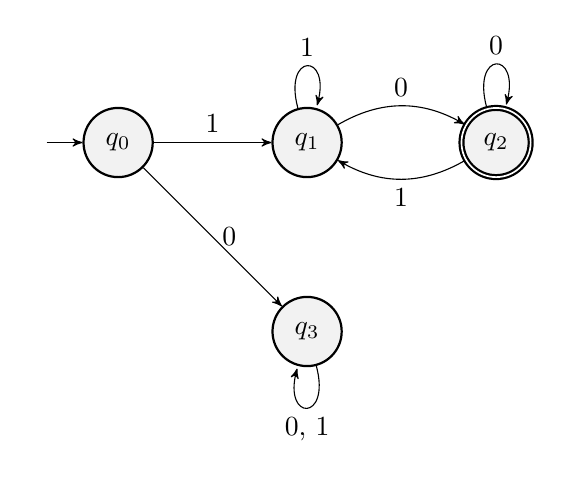
\begin{tikzpicture}
\node[state, initial] (q0) {$q_0$};
\node[state, right of=q0] (q1) {$q_1$};
\node[state, accepting, right of=q1] (q2) {$q_2$};
\node[state, below of=q1] (q3) {$q_3$};
\draw
(q0) edge[below, right] node{0} (q3)
(q0) edge[right, above] node{1} (q1)
(q1) edge[bend left, above] node{0} (q2)
(q1) edge[loop above] node{1} (q1)
(q2) edge[loop above] node{0} (q2)
(q2) edge[bend left, below] node{1} (q1)
(q3) edge[loop below] node{0, 1} (q3)
;
\end{tikzpicture}
}
\item[(c)] $\{w \mid w \textnormal{ contains the substring {\tt 0101} (i.e., $w = x{\tt 0101}y$ for some $x$ and $y$}\}$
\solution{
\if\isanswerkey1\solDFAdiagramsC\fi
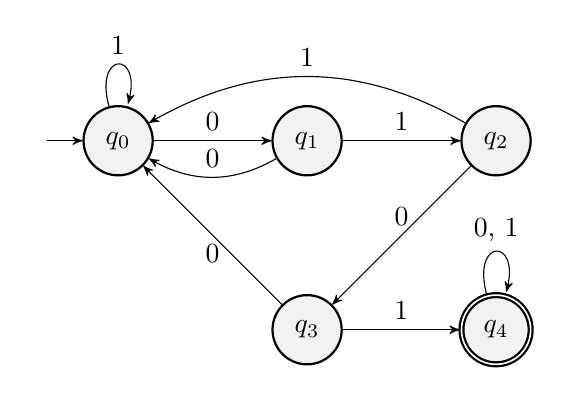
\begin{tikzpicture}
\node[state, initial] (q0) {$q_0$};
\node[state, right of=q0] (q1) {$q_1$};
\node[state, right of=q1] (q2) {$q_2$};
\node[state, below of=q1] (q3) {$q_3$};
\node[state, accepting, right of=q3] (q4) {$q_4$};
\draw
(q0) edge[right, above] node{0} (q1)
(q0) edge[loop above] node{1} (q0)
(q1) edge[bend left, above] node{0} (q0)
(q1) edge[right, above] node{1} (q2)
(q2) edge[right, above] node{0} (q3)
(q2) edge[bend right, above] node{1} (q0)
(q3) edge[left, below] node{0} (q0)
(q3) edge[right, above] node{1} (q4)
(q4) edge[loop above] node{0, 1} (q4)
;
\end{tikzpicture}
}
\item[(d)] $\{w \mid w \textnormal{ has length at least 3 and its third symbol is a {\tt 0}}\}$
\solution{
\if\isanswerkey1\solDFAdiagramsD\fi
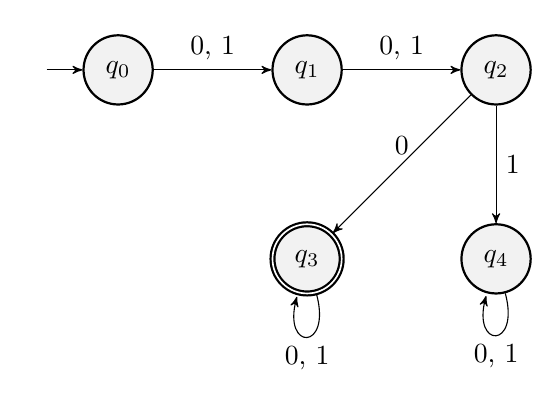
\begin{tikzpicture}
\node[state, initial] (q0) {$q_0$};
\node[state, right of=q0] (q1) {$q_1$};
\node[state, right of=q1] (q2) {$q_2$};
\node[state, accepting, below of=q1] (q3) {$q_3$};
\node[state, right of=q3] (q4) {$q_4$};
\draw
(q0) edge[right, above] node{0, 1} (q1) 
(q1) edge[right, above] node{0, 1} (q2) 
(q2) edge[right, above] node{0} (q3) 
(q2) edge[right, right] node{1} (q4) 
(q3) edge[loop below] node{0, 1} (q3)
(q4) edge[loop below] node{0, 1} (q4)
;
\end{tikzpicture}
}
\item[(e)] $\{w \mid w \textnormal{ starts with {\tt 0} and has odd length, or starts with {\tt 1} and has even length}\}$
\solution{
\if\isanswerkey1\solDFAdiagramsE\fi
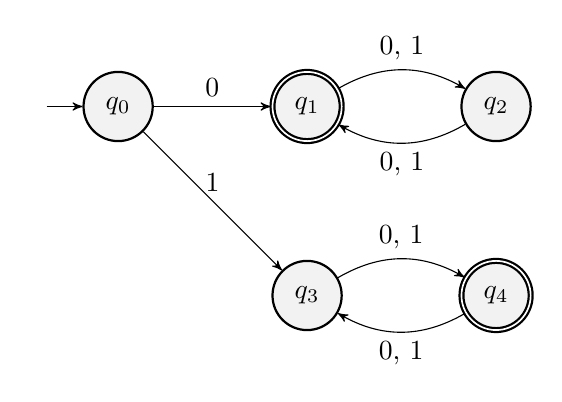
\begin{tikzpicture}
\node[state, initial] (q0) {$q_0$};
\node[state, accepting, right of=q0] (q1) {$q_1$};
\node[state, right of=q1] (q2) {$q_2$};
\node[state, below of=q1] (q3) {$q_3$};
\node[state, accepting, right of=q3] (q4) {$q_4$};
\draw
(q0) edge[right, above] node{0} (q1) 
(q0) edge[right, above] node{1} (q3) 
(q1) edge[bend left, above] node{0, 1} (q2) 
(q2) edge[bend left, below] node{0, 1} (q1) 
(q3) edge[bend left, above] node{0, 1} (q4) 
(q4) edge[bend left, below] node{0, 1} (q3) 
;
\end{tikzpicture}
}
\item[(f)] $\{w \mid w \textnormal{ doesn't contain the substring {\tt 110}}\}$
\solution{
\if\isanswerkey1\solDFAdiagramsF\fi
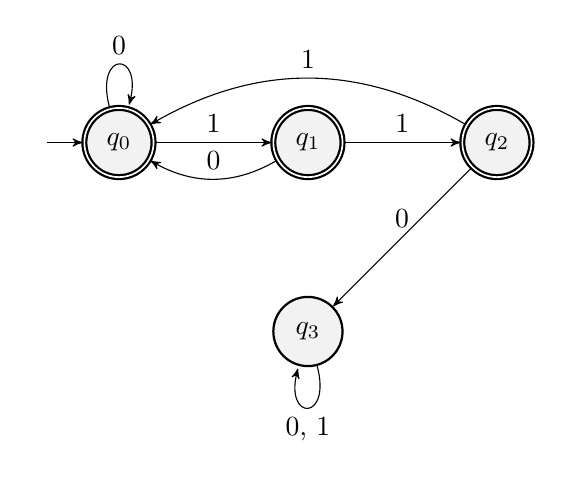
\begin{tikzpicture}
\node[state, accepting, initial] (q0) {$q_0$};
\node[state, accepting, right of=q0] (q1) {$q_1$};
\node[state, accepting, right of=q1] (q2) {$q_2$};
\node[state, below of=q1] (q3) {$q_3$};
\draw
(q0) edge[loop above] node{0} (q0)
(q0) edge[right, above] node{1} (q1)
(q1) edge[bend left, above] node{0} (q0)
(q1) edge[right, above] node{1} (q2)
(q2) edge[right, above] node{0} (q3)
(q2) edge[bend right, above] node{1} (q0)
(q3) edge[loop below] node{0, 1} (q3)
;
\end{tikzpicture}
}
\item[(j)] $\{w \mid w \textnormal{ contains at least two {\tt 0}s and at most one {\tt 1}}\}$
\solution{
\if\isanswerkey1\solDFAdiagramsJ\fi
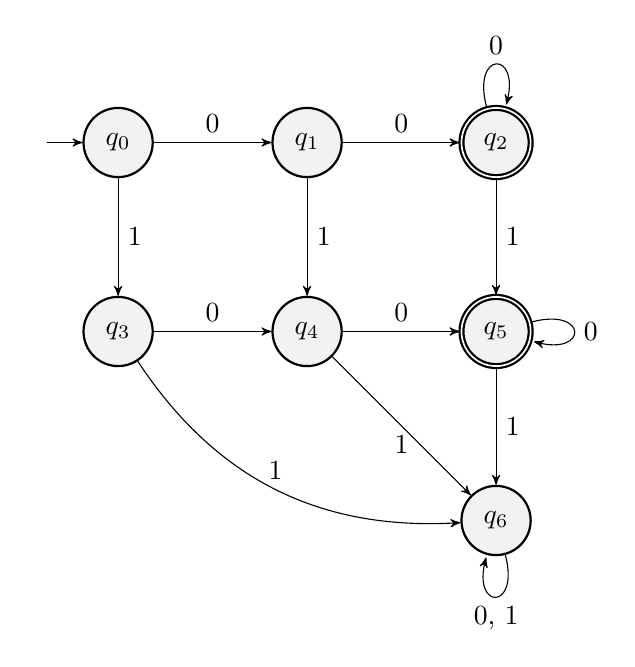
\begin{tikzpicture}
\node[state, initial] (q0) {$q_0$};
\node[state, right of=q0] (q1) {$q_1$};
\node[state, accepting, right of=q1] (q2) {$q_2$};
\node[state, below of=q0] (q3) {$q_3$};
\node[state, right of=q3] (q4) {$q_4$};
\node[state, accepting, right of=q4] (q5) {$q_5$};
\node[state, below of=q5] (q6) {$q_6$};
\draw
(q0) edge[right, above] node{0} (q1)
(q0) edge[right, right] node{1} (q3)
(q1) edge[right, above] node{0} (q2)
(q1) edge[right, right] node{1} (q4)
(q2) edge[loop above] node{0} (q2)
(q2) edge[right, right] node{1} (q5)
(q3) edge[right, above] node{0} (q4)
(q3) edge[bend right, above] node{1} (q6)
(q4) edge[right, above] node{0} (q5)
(q4) edge[right, below] node{1} (q6)
(q5) edge[loop right] node{0} (q5)
(q5) edge[below, right] node{1} (q6)
(q6) edge[loop below] node{0, 1} (q6)
;
\end{tikzpicture}
}
\item[(m)] The empty set
\solution{
\if\isanswerkey1\solDFAdiagramsM\fi
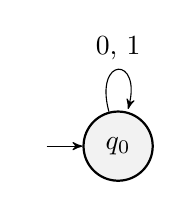
\begin{tikzpicture}
\node[state, initial] (q0) {$q_0$};
\draw
(q0) edge[loop above] node{0, 1} (q0);
\end{tikzpicture}
}
\item[(n)] All strings except the empty string
\solution{
\if\isanswerkey1\solDFAdiagramsN\fi
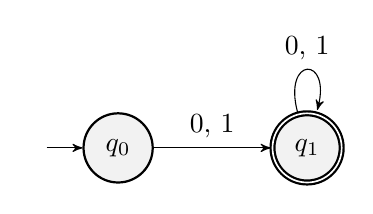
\begin{tikzpicture}

\node[state, initial] (q0) {$q_0$};
\node[state, accepting, right of=q0] (q1) {$q_1$};
\draw
(q0) edge[right, above] node{0, 1} (q1)
(q1) edge[loop above] node{0, 1} (q1);
\end{tikzpicture}
}

\end{enumerate}





\end{enumerate}


\end{document}
